\documentclass{beamer}
\setbeamertemplate{navigation symbols}{}

\usepackage{beamerthemeshadow}
\setbeamertemplate{caption}[numbered]

\hypersetup{colorlinks}

\def\gw#1{gravitational wave#1 (GW#1)\gdef\gw{GW}}
\def\ns#1{neutron star#1 (NS#1)\gdef\ns{NS}}

\newcommand{\red}[1]{{\color{red}{#1}}}

\begin{document}
\title{NS Group Update}
\subtitle{Burst Call Oct 8$^{\text{th}}$ 2014}  
\author{James A. Clark}
\institute{Georgia Institute Of Technology}
\date{} 

\begin{frame}[plain]
\titlepage
\end{frame}

\begin{frame}\frametitle{Table of contents}\tableofcontents
\end{frame} 

\section{NS Group}

\begin{frame}
    \frametitle{The Group}
    Joining the group:
    \begin{itemize}
        \item Calls: bi-weekly, Friday 11am EST, burst TeamSpeak channel
        \item
            {\small\href{https://wiki.ligo.org/viewauth/GIANT/GIANTteleconAgendas}
            {https://wiki.ligo.org/viewauth/GIANT/GIANTteleconAgendas}}
        \item Call time negotiable!
        \item External speakers to resume soon, watch this space\dots
    \end{itemize}
    Scope:
    \begin{itemize}
        \item Explore / discuss astrophysics \& data analysis strategies
            pertaining to transient, unmodelled \gw{} bursts from \ns{s}
    \end{itemize}
    Projects:
    \begin{itemize}
        \item Magnetar QPOs (Quitzow-James)
        \item Post-BNS bursts (Clark, Pannarale)
        \item \dots others welcome!
    \end{itemize}
\end{frame}

\section{NS Search Proposal Highlights}

\begin{frame}
    \frametitle{NS Search Proposal}
    Search proposal nearing completion:
    \begin{itemize}
        \item Current draft in DCC: {\small \href{https://dcc.ligo.org/LIGO-T1400606}{https://dcc.ligo.org/LIGO-T1400606}}
        \item DAC SVN:
            {\small \href{https://trac.ligo.caltech.edu/dac/browser/WhitePaper/2014-2015}
            {https://trac.ligo.caltech.edu/dac/browser/WhitePaper/2014-2015}}
    \end{itemize}
    For O1 plan is to only target \emph{extraordinary} events:
    \begin{itemize}
        \item Hyper-flares from Galactic magnetars (c.f., SGR 1806-20)
        \item Targeted, high-frequency PE follow-up for BNS
    \end{itemize}
    Highly speculative sources, but rare occurrences, huge
    science potential, minimal resource requirements \& build off or use
    analyses which are either mature or under development anyway.
\end{frame}

\subsection{Galactic Magnetar Hyperflares}
\begin{frame}
    \frametitle{Galactic Hyperflares: science case}
    \begin{itemize}
        \item LSC/Virgo have a history of high-profile, astrophysically interesting
            searches for \gw{s} associated with magnetar flaring activity

        \item O1 will probably not dramatically improve upon these results for
            normal flaring activity

        \item However, recall SGR 1806-20: $10^{47}$\,erg in hard X-rays / soft $\gamma$-rays in
            $<1$\,s, \emph{within our Galaxy}

        \item An event of this nature would generate significant astrophysical
            interest and may excite various \ns{} oscillation modes; we
            should be prepared to say something
    \end{itemize}
\end{frame}

\begin{frame}
    \frametitle{Galactic Hyperflares: search method}
    \begin{itemize}
        \item Magnetar hyperflares are similar to short-GRBs.  Seems likely that
            this would already trigger the low-latency GRB analyses.
        \item Propose: analysis with SNEWS-like configuration of
            \textsc{X-Pipeline} (but Swift-like sky-grid)
        \item Minimises development requirements, extends to higher frequencies
            than standard GRB analysis, shorter on-source window
        \item Only a small chance ($\sim 1\%$) of occurrence \& standard GRB
            analysis would very likely run anyway! 
        \item Development required: automatic selection of appropriate
            \textsc{X-Pipeline} configuration for SGR triggers
        \item Alternatively: maximum of 1 re-analysis after automated GRB
            analysis with SNEWS-configuration
    \end{itemize}
\end{frame}

\begin{frame}
    \frametitle{Galactic Hyperflares: Publication Plan}
    \begin{itemize}
        \item {\bf Confident Detection} ($>3\sigma$): report detection \&
            spectral analysis of waveform as reconstructed by (e.g.,)
            \textsc{BayesWave}
        \item {\bf Marginal Detection} (2--3$\sigma$): report candidate \&
            present waveform reconstruction / spectrum with less emphasis
        \item {\bf No Detection}: only publish if ratio of \gw{} energy U.L. to
            isotropic EM energy is \emph{significantly} lower (better) than all
            past magnetar analyses.  Otherwise, non-detection statement in e.g.,
            end-of-run GRB publication (?)
    \end{itemize}
\end{frame}

\subsection{Post-BNS Bursts}
%\begin{frame}
%    \tableofcontents[currentsection,currentsubsection]
%\end{frame}

\begin{frame}
    \frametitle{Postmerger Bursts: science case}
    \begin{itemize}
        \item Likely outcome of BNS coalescence: formation of (quasi) stable,
            differentially rotating, oscillating \ns{} remnant
        \item 10--100\,ms, 1--4\,kHz \gw{} emission, detectable in aLIGO (ZDHP) to
            few--10's of Mpc (depending on data analysis strategy, degree of
            damping, stability of remnant, \dots)
        \item Detection \& frequency estimation can constrain \ns{} equation of
            state
        \item Not \emph{likely} to be detectable in O1
        \item BUT astrophysics potential is enormous \& merger/post-merger signal is
            exclusively burst-science, inaccessible to matched-filtering
        \item Plausible first detection scenario: BNS inspiral; questions
            \emph{will} be asked about the post-merger!
    \end{itemize}
\end{frame}

\begin{frame}
    \frametitle{Postmerger Bursts: search method}
    \begin{itemize}
        \item Post-merger analysis $\iff$ inspiral detection.
        \item Minimum: correlation of all-sky HF triggers (and reconstructions)
            with inspiral time of coalescence $t_c \pm 100$\,ms
        \item Nominal: targeted follow-up of inspiral trigger with
            \textsc{BayesWave} / \textsc{LIB}
        \item Targeted: narrow time-window around $t_c$, high-frequency
            (1--4\,kHz), possibly also restricted sky-location from inspiral
            sky-map
    \end{itemize}
    Some development is required and underway:
    \begin{itemize}
        \item Formalize simulation infrastructure for post-merger waveforms
        \item Tune time/frequency parameter space
    \end{itemize}
\end{frame}

\begin{frame}
    \frametitle{Postmerger Bursts: Publication Plans}
    \begin{itemize}
        \item {\bf Confident \& Marginal Detections}: any detection of a
            post-merger BNS signal will be ground-breaking.  A confident
            detection will give higher fidelity reconstruction and spectral
            analysis, but marginal detection alone indicates survival against
            prompt-collapse.  Publish either to accompany CBC deep P.E.
        \item {\bf No detection}: Degeneracy between prompt-collapse \&
            surviving but distant post-merger \ns{} renders upper limits
            somewhat unininteresting; ``no evidence for a post-merger signature
            was observed'' in the inspiral detection paper would suffice.
    \end{itemize}
\end{frame}

\begin{frame}
    \frametitle{Postmerger Bursts: Resource Requirements}
    Work in progress but note:
    \begin{itemize}
        \item Expect $<1$ event to follow-up
        \item Exceedingly small ``on-source'' time required, thanks to inspiral
            measurement
        \item Confident of single-core follow-up in $\lesssim 1$\,hr
        \item Cost will be dominated by development \& tuning
    \end{itemize}
\end{frame}


\section{Project News} 
\begin{frame}\tableofcontents[currentsection]
\end{frame}

\subsection{Magnetar QPOs}
\begin{frame}\frametitle{Magnetar QPOs} 
\end{frame}


\subsection{Post-BNS Bursts}
\begin{frame}\frametitle{Postmerger Injection Data \& Infrastructure} 
    Collaboration with A. Bauswein et al: quadrupole moments for variety of
    numerical post-merger waveforms (e.g.,
    \href{http://arxiv.org/abs/1406.5444}{arXiv:1406.5444})\footnote{Note that B.
    Giacomazzo also has publicly available waveforms}
    \begin{itemize}
        \item Can construct waveform polarizations $h_{+,\times}$ following
            \href{https://dcc.ligo.org/cgi-bin/private/DocDB/ShowDocument?.submit=Number&docid=T1000553&version=}{T1000553}
        \item Python scripts which mimic the \textsc{NINJA} MDC codes but use
            \textsc{SWIG}-wrapped \textsc{LALSimulation} to project waveforms onto
            detector network approaching maturity
        \item Currently used as a wrapper for \textsc{LIB} studies with
            on-the-fly MDC frames but trivial modification for MDC frame
            generation 
    \end{itemize}
\end{frame}

\begin{frame}
    \frametitle{\textsc{LIB} templates for post-merger signals}

    \begin{figure}
        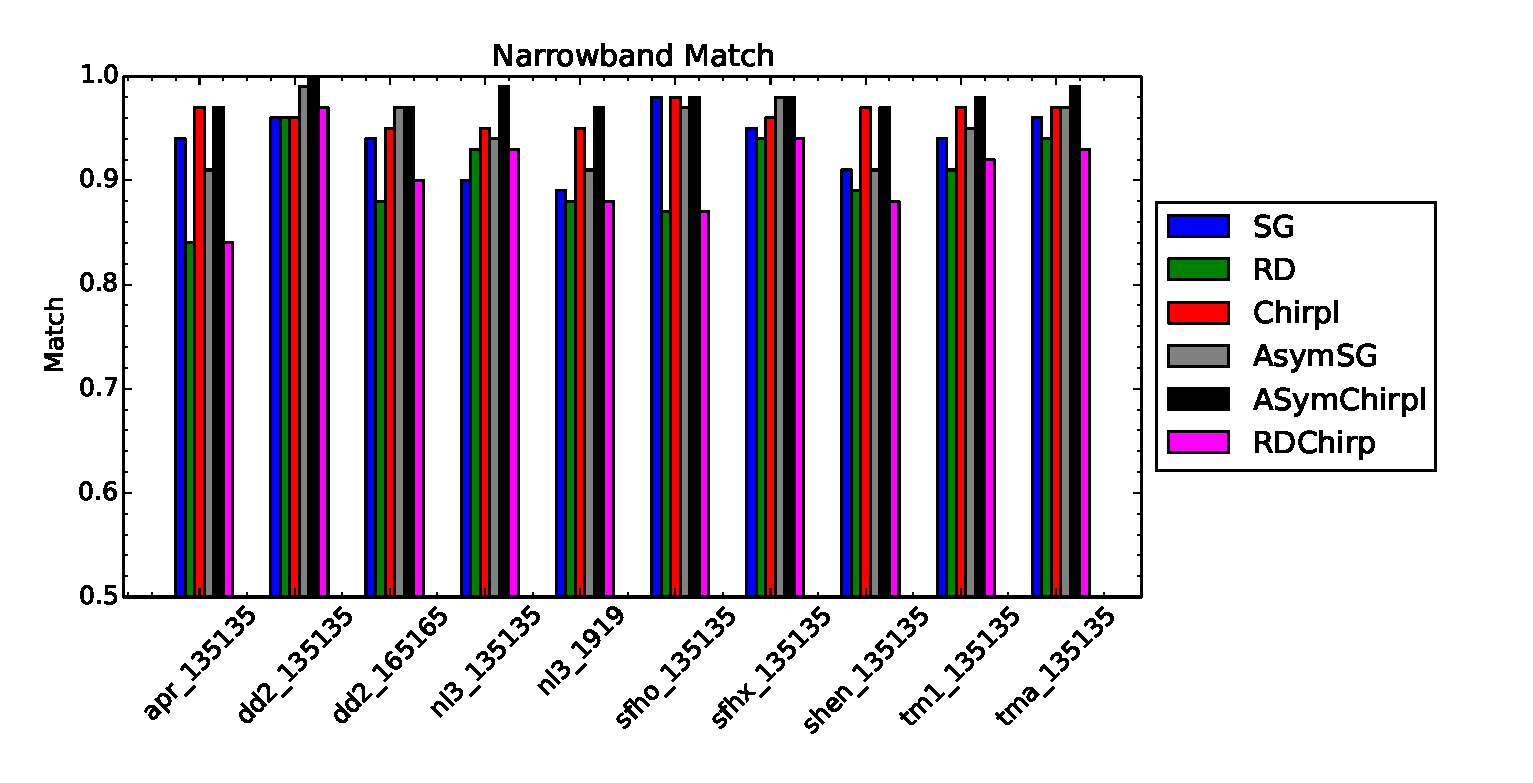
\includegraphics[scale=0.4]{nb_match.eps} 
        \caption{Match for ad hoc burst templates for a collection of
        post-merger waveforms.  Note that match calculation is restricted to frequency
    band of dominant post-merger oscillation.}
    \end{figure}

\end{frame}

\begin{frame}
    \frametitle{\textsc{LIB} Post-merger Frequency Estimation}

    \begin{figure}
        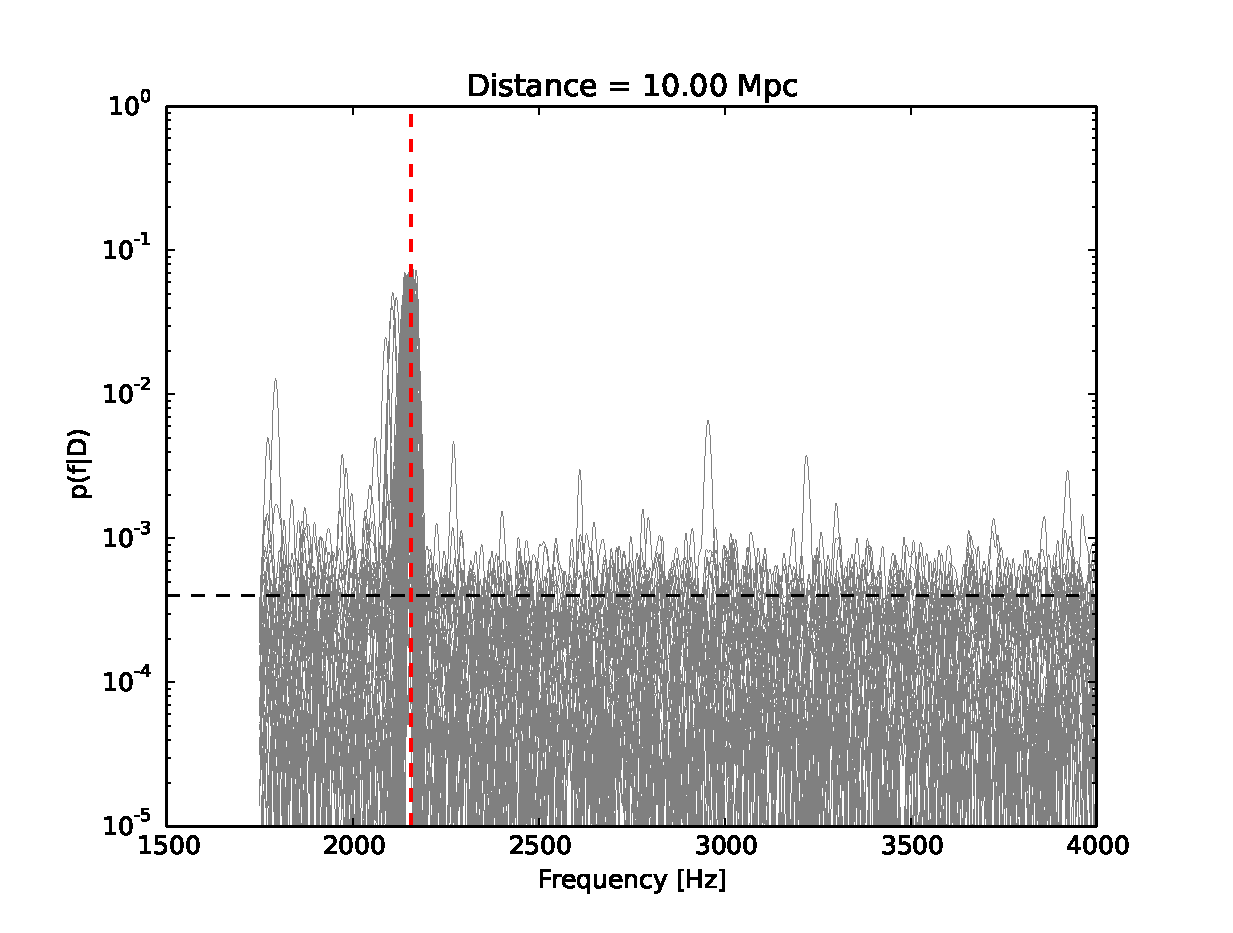
\includegraphics[scale=0.35]{freqpdflines_dist-10_00.eps} 
        \caption{\textsc{LIB} marginal frequency posteriors (sine-Gaussians) for
        an ensemble of post-merger waveform (fixed EOS) at 10\,Mpc.}
    \end{figure}

\end{frame}

\begin{frame}
    \frametitle{\textsc{BayesWave} for post-merger signals}
    Exploratory studies are also beginning in the use of \textsc{BayesWave}.
    {\bf Preliminary} results pages for default BW configuration, single-IFO
    injections:
    \begin{itemize}
        \item {\small
    \href{https://ldas-jobs.ligo.caltech.edu/~francesco.pannarale/BayesWaveRuns/HMNS/}{https://ldas-jobs.ligo.caltech.edu/\textasciitilde{}francesco.pannarale/BayesWaveRuns/HMNS/}}
    \end{itemize}

    \begin{columns}[]
        \column{0.5\textwidth}
        \begin{figure}
            \vspace*{-0.5cm}

            \begin{center}
                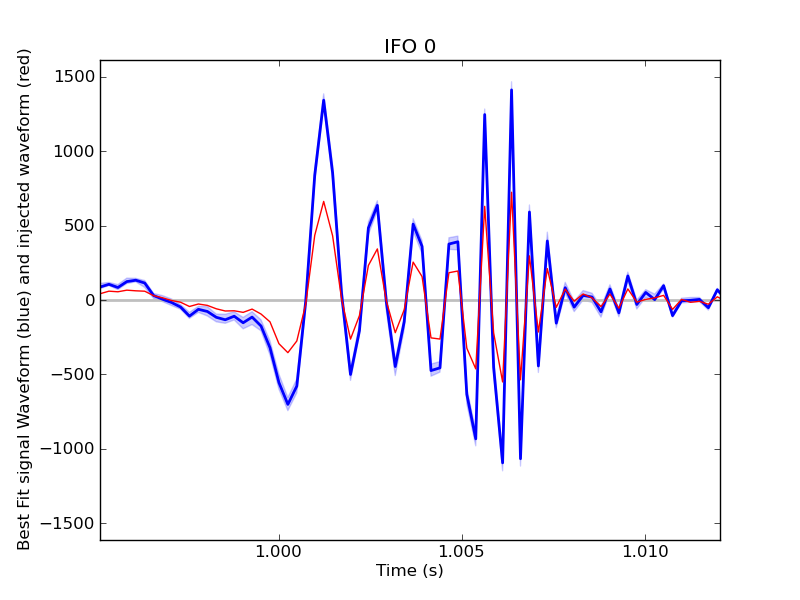
\includegraphics[scale=0.3]{signal_waveform_0.png} 
                %\caption{Example \textsc{BayesWave} injection/reconstruction.
                %Default BW configuration appears to have downsampled the
%            injection and washed out the post-merger; tuning begins!}
            \end{center}

        \end{figure}

        \column{0.5\textwidth}

        \begin{block}{Example \textsc{BayesWave} injection/reconstruction}
            Default BW configuration appears to have downsampled the
            injection but overlap looks good; tuning begins!
        \end{block}


    \end{columns}

\end{frame}

\begin{frame}
    \frametitle{Summary}
    Main news:
    \begin{itemize}
        \item NS search plan draft very nearly complete.  Discussion extremely welcome!
    \end{itemize}
    Projects news:
    \begin{itemize}
        \item Magnetar QPOs:
        \item Post-BNS bursts: injection infrastructure \& PE wrapper scripts
            under development; tuning and optimization of
            \textsc{BayesWave}/\textsc{LIB} now underway
    \end{itemize}
    Again, new projects and additional effort very, very welcome!
\end{frame}




\end{document}
